\section{Diseño detallado}

\subsection{Accionamiento mecánico}
\subsubsection{Propuestas para el movimiento lineal}
Primero se estableció el perfil de movimiento del sistema, en este caso se considera un perfil trapezoidal, como el que se muestra en la \emph{figura}\ref{fig:perfil_movi} con tiempos de espera $t_{dwell}\approx 0$, mientras que los tiempos de aceleración, desaceleración y de velocidad pico se consideraron iguales. $t_1 = t_2 = t_3$.
Tomando los requerimientos de movimiento y fuerza de la \emph{tabla}\ref{tab:cuadro_rf} establecemos que: $V_{pk} = 1000 mm/s$, $S = 400mm$, $m_L = 20Kg$.
\begin{center}
    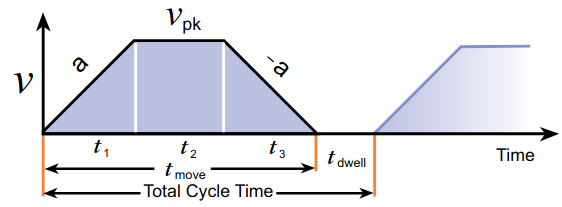
\includegraphics[scale=0.55]{imagenes/Perfil de movimiento.png}
    \captionof{figure}{Perfil de movimiento del eje lineal}
    \label{fig:perfil_movi}
\end{center}

\underline{Propuesta 1}
\\La primera propuesta es un mecanismo de tornillo sin fin de $d = 10mm$ y con una velocidad angular máxima de $2000 rpm$ \\
\newline
\textbf{Tiempo de recorrido}
\begin{equation}
    t = \frac{3S}{2V_{pk}} = \frac{3(0.4m)}{2(1m/s)} = 0.6s
\end{equation}

\textbf{Aceleración lineal}
\begin{equation}
    a = \frac{V_f-V_i}{t_1} = \frac{1m/s-0m/s}{0.2s}=5m/s^2
\end{equation}

\textbf{Cálculo del paso del tornillo}
\begin{equation}
    L_{min}=\frac{60V_{pk}}{n}=\frac{60(1m/s)}{2000RPM}=0.03m/rev = 30mm/rev
\end{equation}
De la tabla\ref{fig:tornillos_ke} de tornillos Kerk obtenemos que el valor comercial más cercano para $D(\phi)=10mm$. Con esto determinamos que:
\begin{equation}
    L = 30.48 mm/rev = 0.03
\end{equation}
con $\eta = 0.84$ y $J_s = 1.6\times 10^{-6} Kgm^2$
\begin{center}
    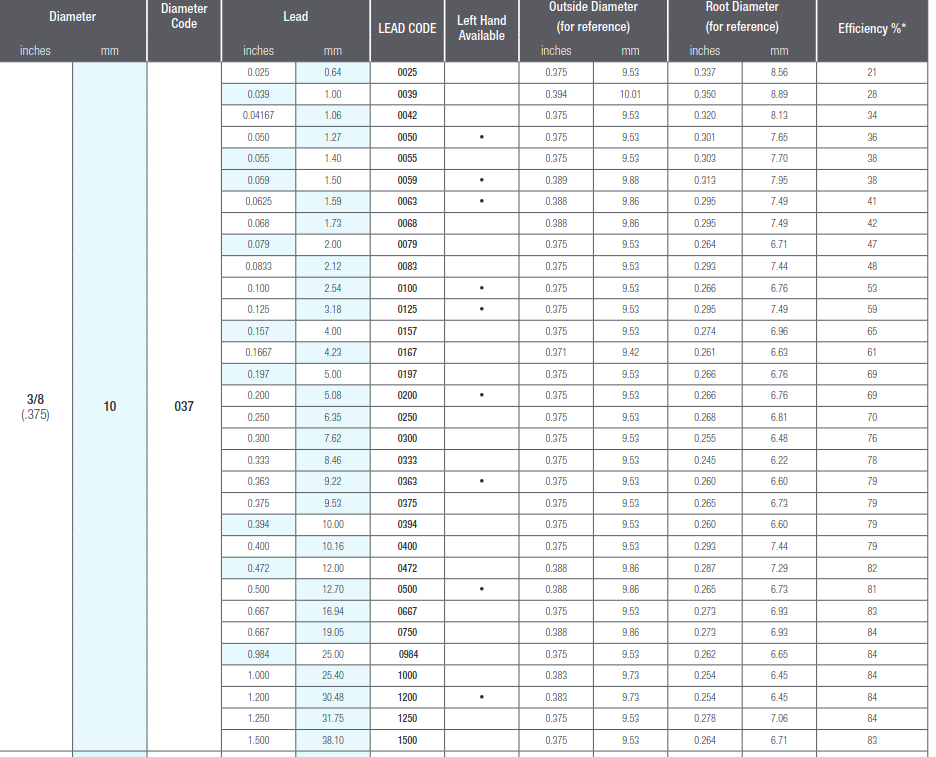
\includegraphics[scale=0.4]{imagenes/tornillos kerk.png}
    \captionof{figure}{Sección del catálogo de tronillos Kerk}
    \label{fig:tornillos_ke}
\end{center}
\textbf{Velocidad angular}
\begin{equation}
    \omega_{pk}=\frac{2\pi V_{pk}}{L}=\frac{2\pi (1 m/s)}{0.03048 m/rev} = 206.14rad/s
\end{equation}
\textbf{Aceleración angular}
\begin{equation}
    \alpha = \frac{2\pi a}{L}=\frac{2\pi (5m/s^2)}{0.03048}=1030.70rad/s^2
\end{equation}
\textbf{Inercia}
\begin{equation}
    J_{in}=m_L(\frac{L}{2\pi})^2\frac{1}{\eta}+J_s=(20Kg)(\frac{0.030348m}{2\pi})^2\frac{1}{0.84}+1.6\times 10^{-6}Kgm^2=5.62\times 10^{-4}Kgm^2
\end{equation}
\textbf{Torque}
\begin{align}
    T_{in}=T_a + T_f + T_g + T_D \\
    T_a = J_{in}\alpha_{in}=(5.62\times 10^{-4})(1030.70)(1.2)=0.6951Nm \\
    T_f = \frac{m_Lg\mu L}{2\pi \eta}=\frac{20(9.81)(0.3)(0.03048)}{2\pi (0.84)}=0.3399Nm \\
    T_g = \frac{m_LgLsen\phi}{2\pi \eta}=0Nm \\
    T_D = 0
\end{align}
\begin{center}
    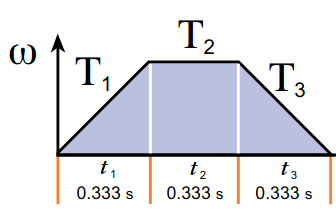
\includegraphics[scale=0.55]{imagenes/perfil torque.png}
    \captionof{figure}{Gráfica de velociad vs tiempo indicando el torque requerido en el movimiento}
    \label{fig:perfil_torq}
\end{center}
Calculamos el torque requerido para la aceleración, desaceleración y en velocidad constante, considerando un factor de seguridad de 1.5:
\begin{align}
    T_1 = T_3 = (T_a+T_f+T_g+T_D)(F.S)\\
    = (0.6951+0.3399+0+0)(1.5) = 1.5525Nm \\
    T_2 = (T_a+T_f+T_g+T_D)(F.S) \\
    = (0+0.3399+0+0)(1.5)=0.5098Nm
\end{align}
\textbf{Torque RMS}
\begin{equation}
    T_{RMS}=\sqrt{\frac{T_1^2t_1+T_2^2t_2+T_3^2t_3}{t_1+t_2+t_3+t_d}} = 1.3013Nm
\end{equation}
\textbf{Potencias}
\begin{align}
    P_1 = P_3 = T_1\omega_{pk} = 320.03W \\
    P_2 = T_2\omega{pk}=105.09W
\end{align}

\underline{Propuesta 2}
\\Ahora se propone un mecanismo de correa y poleas para el movimiento lineal, nuevamente se limitaran las RPM a 2000. El tiempo de recorrido y la aceleración lineal de las ecuaciones (1) y (2) son las mismas.
\\
\newline
\textbf{Diámetro de la polea}
\begin{equation}
    D=\frac{60V_{pk}}{n\pi}=\frac{60(1m/s)}{2000RPM\pi}=9.54mm
\end{equation}
De la tabla\ref{fig:poleas} de poleas obtenemos que el valor comercial más cercano para $D=9.54mm$ es $D=9.55mm$
\begin{equation}
    m_p = \rho_{alum}W\frac{\pi D^2}{4}=1.78\times 10^{-3}Kg
\end{equation}
\begin{center}
    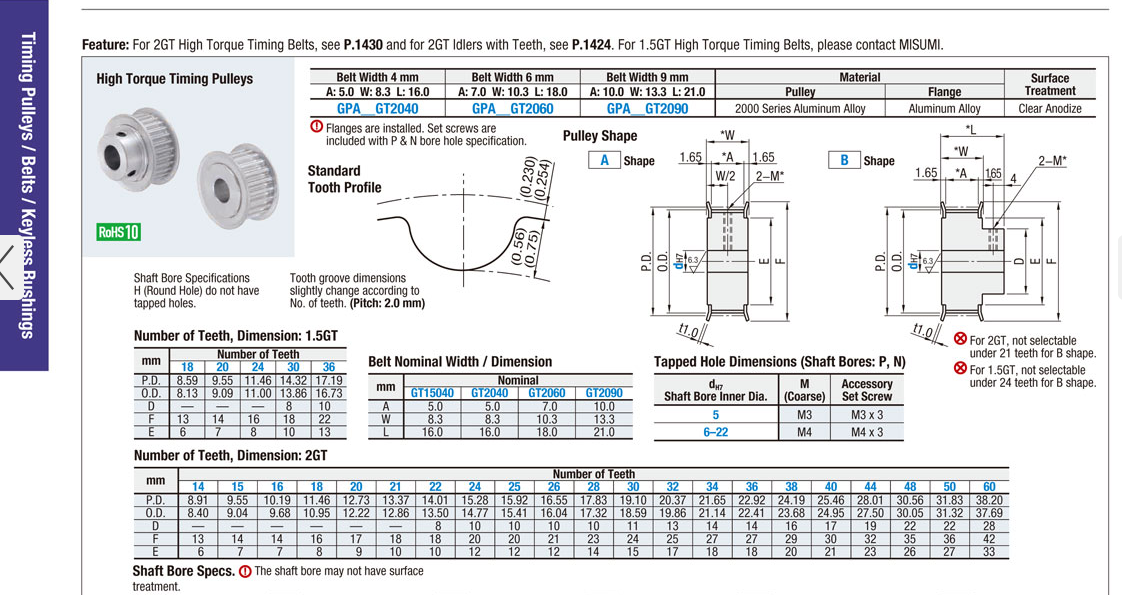
\includegraphics[scale=0.4]{imagenes/catalogo poleas.png}
    \captionof{figure}{Sección del catálogo de poleas}
    \label{fig:poleas}
\end{center}
\textbf{Velocidad angular}
\begin{equation}
    \omega_{pk}=\frac{60V_{pk}}{\pi D}=\frac{60(1)}{\pi (9.55)} = 209.42rad/s
\end{equation}
\textbf{Aceleración angular}
\begin{equation}
    \alpha = \frac{\omega_f-\omega_o}{t_1}=\frac{209.42-0}{0.2}=1047.1rad/s^2
\end{equation}
\textbf{Inercia}
\begin{align}
    J_{L}=\frac{m_LD^2}{4}=\frac{(20)(9.04)^2}{4}=4.086\times 10^{-4}Kgm^2 \\
    J_p = \frac{m_pD^2}{8}=\frac{1.78\times 10^{-3}(9.04)}{8} = 1.818\times 10^{-8}Kgm^2 \\
    J_T = (J_L+2J_p)(1.01)=(4.086\times 10^{-4})(2)(1.818\times 10^{-8})(1.01)=4.127\times 10^{-4}Kgm^2
\end{align}
\textbf{Torque}
\begin{align}
    T_a = J_{T}\alpha=(4.127\times 10^{-4})(1.2)=0.5185Nm \\
    T_L = \frac{m_LgD(sen\alpha+\mu cos\alpha)}{2 \eta}=\frac{20(9.81)(0.3)(9.55)}{2(0.85)}=0.3306Nm \\
\end{align}
Calculamos el torque requerido para la aceleración, desaceleración y en velocidad constante, considerando un factor de seguridad de 1.5:
\begin{align}
    T_1 = T_3 = (T_a+T_L)(F.S)\\
    = (0.5185+0.3306)(1.5) = 1.2736Nm \\
    T_2 = (T_L)(F.S) \\
    = (0.3306)(1.5)=0.4959Nm
\end{align}
\textbf{Torque RMS}
\begin{equation}
    T_{RMS}=\sqrt{\frac{T_1^2t_1+T_2^2t_2+T_3^2t_3}{t_1+t_2+t_3+t_d}} = 1.0785Nm
\end{equation}
\textbf{Potencias}
\begin{align}
    P_1 = P_3 = T_1\omega_{pk} = 320.03W \\
    P_2 = T_2\omega{pk}=105.09W
\end{align}